\documentclass[11pt]{article}
\usepackage[a4paper,margin=2.5cm]{geometry}
\usepackage{amsmath,amssymb,amsthm,graphicx,booktabs,xcolor}
\usepackage[colorlinks=true,linkcolor=blue!60!black,citecolor=blue!60!black,urlcolor=blue!60!black]{hyperref}
\usepackage{xurl}
\hypersetup{pdftitle={Renormalization Group Flows of Spectral Dimensions on Hierarchical Lattices},pdfauthor={Ruqing Chen}}
\setlength{\emergencystretch}{3em}
\graphicspath{{../figures/}{figures/}{./}}

\newtheorem{theorem}{Theorem}
\newtheorem{proposition}{Proposition}[section]
\newtheorem{lemma}{Lemma}[section]
\theoremstyle{remark}\newtheorem*{remark}{Remark}

\newcommand{\dd}{\mathrm{d}}
\newcommand{\ZZ}{\mathbb{Z}}
\newcommand{\EE}{\mathbb{E}}
\newcommand{\paperdoi}{10.5281/zenodo.23201028}

\title{Renormalization Group Flows of Spectral Dimensions\\ on Hierarchical Lattices: Critical Percolation,\\ Resistance Exponents, and Transport Universality}
\author{Ruqing Chen\\[2pt]
\small GUT Geoservice Inc., Montreal, Quebec, Canada\\
\small \href{mailto:ruqing@hotmail.com}{\texttt{ruqing@hotmail.com}}}
\date{\small DOI: \href{https://doi.org/\paperdoi}{\paperdoi}}

\begin{document}
\maketitle

\begin{abstract}
A recurring idea in discrete approaches to quantum gravity and in network models of growth is that coarse-graining
drives a graph \emph{spontaneously} to a stable non-integer spectral dimension. We test this idea on a model in which
the renormalization group (RG) is exact: bond percolation on the diamond hierarchical lattice (DHL).

The edge-retention probability obeys $p'=2p^2-p^4$. This map has two attracting fixed points, $p=0$ (fragmented,
$d_s\to0$) and $p=1$ (intact lattice, $d_s=2$), and one repulsive fixed point $p_c=(\sqrt5-1)/2$, with
$\nu=\ln2/\ln(6-2\sqrt5)\approx1.6353$. A non-integer spectral dimension therefore appears only at a tuned, unstable
critical point. For the critical spanning cluster, including all dangling parts, the conditional moments of the
cluster mass obey an exact $2\times2$ linear recursion. Its Perron eigenvalue $\Lambda=7-2\sqrt5+\sqrt{73-32\sqrt5}$ gives
the closed-form mass dimension $d_f=\log_2\Lambda=1.89929$. Population dynamics reproduces it to $0.1\%$ after twenty
levels. The resistance between the poles obeys a nonlinear recursion with Lyapunov exponent $\zeta=0.8127\pm0.0002$, so
the Einstein relation gives $d_s=2d_f/(d_f+\zeta)\approx1.401$. Exact diagonalisation of the graph Laplacian on generations~6
and~7, averaged over whole log-periods, gives $1.41$ and $1.44$. The same procedure gives $1.994$ for the intact lattice,
whose exact value is $2$.

Away from $p_c$, $d_s(\tau)$ crosses over to $0$ or $2$ beyond $\xi\sim|p-p_c|^{-\nu}$. Newman--Watts shortcuts are a relevant
perturbation that raises $d_s$ beyond $\tau\sim\xi^2$ without creating a plateau. The DHL critical cluster has nearly the
mass dimension of two-dimensional percolation, $91/48=1.8958$, but a very different resistance exponent ($0.813$ versus
$0.983$). Its spectral dimension, about $1.40$, therefore differs from the $\ZZ^2$ value $1.317$, from the mean-field value
$4/3$, and from the value $1.25$ sometimes assumed. Geometric similarity does not imply a common transport universality
class. The spectral dimension of ``the critical cluster'' also depends on the chosen subgraph and Laplacian, as the
comparison with the Hambly--Kumagai diffusion shows.
\end{abstract}

\tableofcontents

%=====================================================================
\section{Introduction}
\label{sec:intro}

Several approaches to quantum gravity find that the effective dimension of spacetime, measured by the spectral
dimension of a diffusion process, depends on scale~\cite{AJL,Carlip}. Similar scale-dependent dimensions occur in
disordered media and on fractals~\cite{BenAvrahamHavlin}. In earlier work we showed that the
spectral dimension is an equipartition count, $d_s(\tau)=2\tau\langle\lambda\rangle_\tau$, and that physical values must be
read from scaling windows between cutoff effects~\cite{Chen2026_qgc}. Here we ask how $d_s$ flows under an exact
coarse-graining of a graph.

A tempting picture is that a discrete network, under a renormalization of its connectivity, undergoes a topological
transition in which its spectral dimension ``spontaneously jumps'' from an integer to a stable non-integer value.
A specific value such as $d_s\approx1.25$ is sometimes posited for the resulting fractal, but we are not aware of a
derivation of it. For comparison, generic branched polymers, the tree-like phase of two-dimensional quantum gravity,
have $d_s=4/3$~\cite{JonssonWheater}. Three statements in this picture can be tested.
\begin{enumerate}
\item Is the non-integer fixed point attractive, i.e.\ reached spontaneously?
\item Is the change of $d_s$ a jump?
\item What is the value of $d_s$ at the critical point, and is it universal?
\end{enumerate}
Hierarchical lattices make the RG exact~\cite{BerkerOstlund,KaufmanGriffiths}. On the diamond hierarchical lattice the
percolation transition and its scaling limit are understood rigorously~\cite{HamblyKumagai}. Our answers are no; no,
it is a crossover; and approximately $1.40$ for the full critical cluster, which is not universal across lattices,
subgraphs or Laplacians.

\paragraph{Main results.}
\begin{itemize}
\item The mass dimension of the critical spanning cluster, including dangling parts, has the closed form
$d_f=\log_2\bigl(7-2\sqrt5+\sqrt{73-32\sqrt5}\bigr)=1.89929$ (Theorem~\ref{thm:mass}).
\item The resistance exponent is $\zeta=0.8127\pm0.0002$. Together with the Einstein relation and exact diagonalisation,
this gives $d_s\approx1.40$--$1.44$ (Section~\ref{sec:ds}).
\item Off-critical and rewired graphs flow away from the critical value (Section~\ref{sec:stability}).
\item Two-dimensional percolation and the DHL share the mass dimension to $0.2\%$, but not the transport exponents
(Section~\ref{sec:universality}).
\end{itemize}

\begin{figure}[t]
\centering
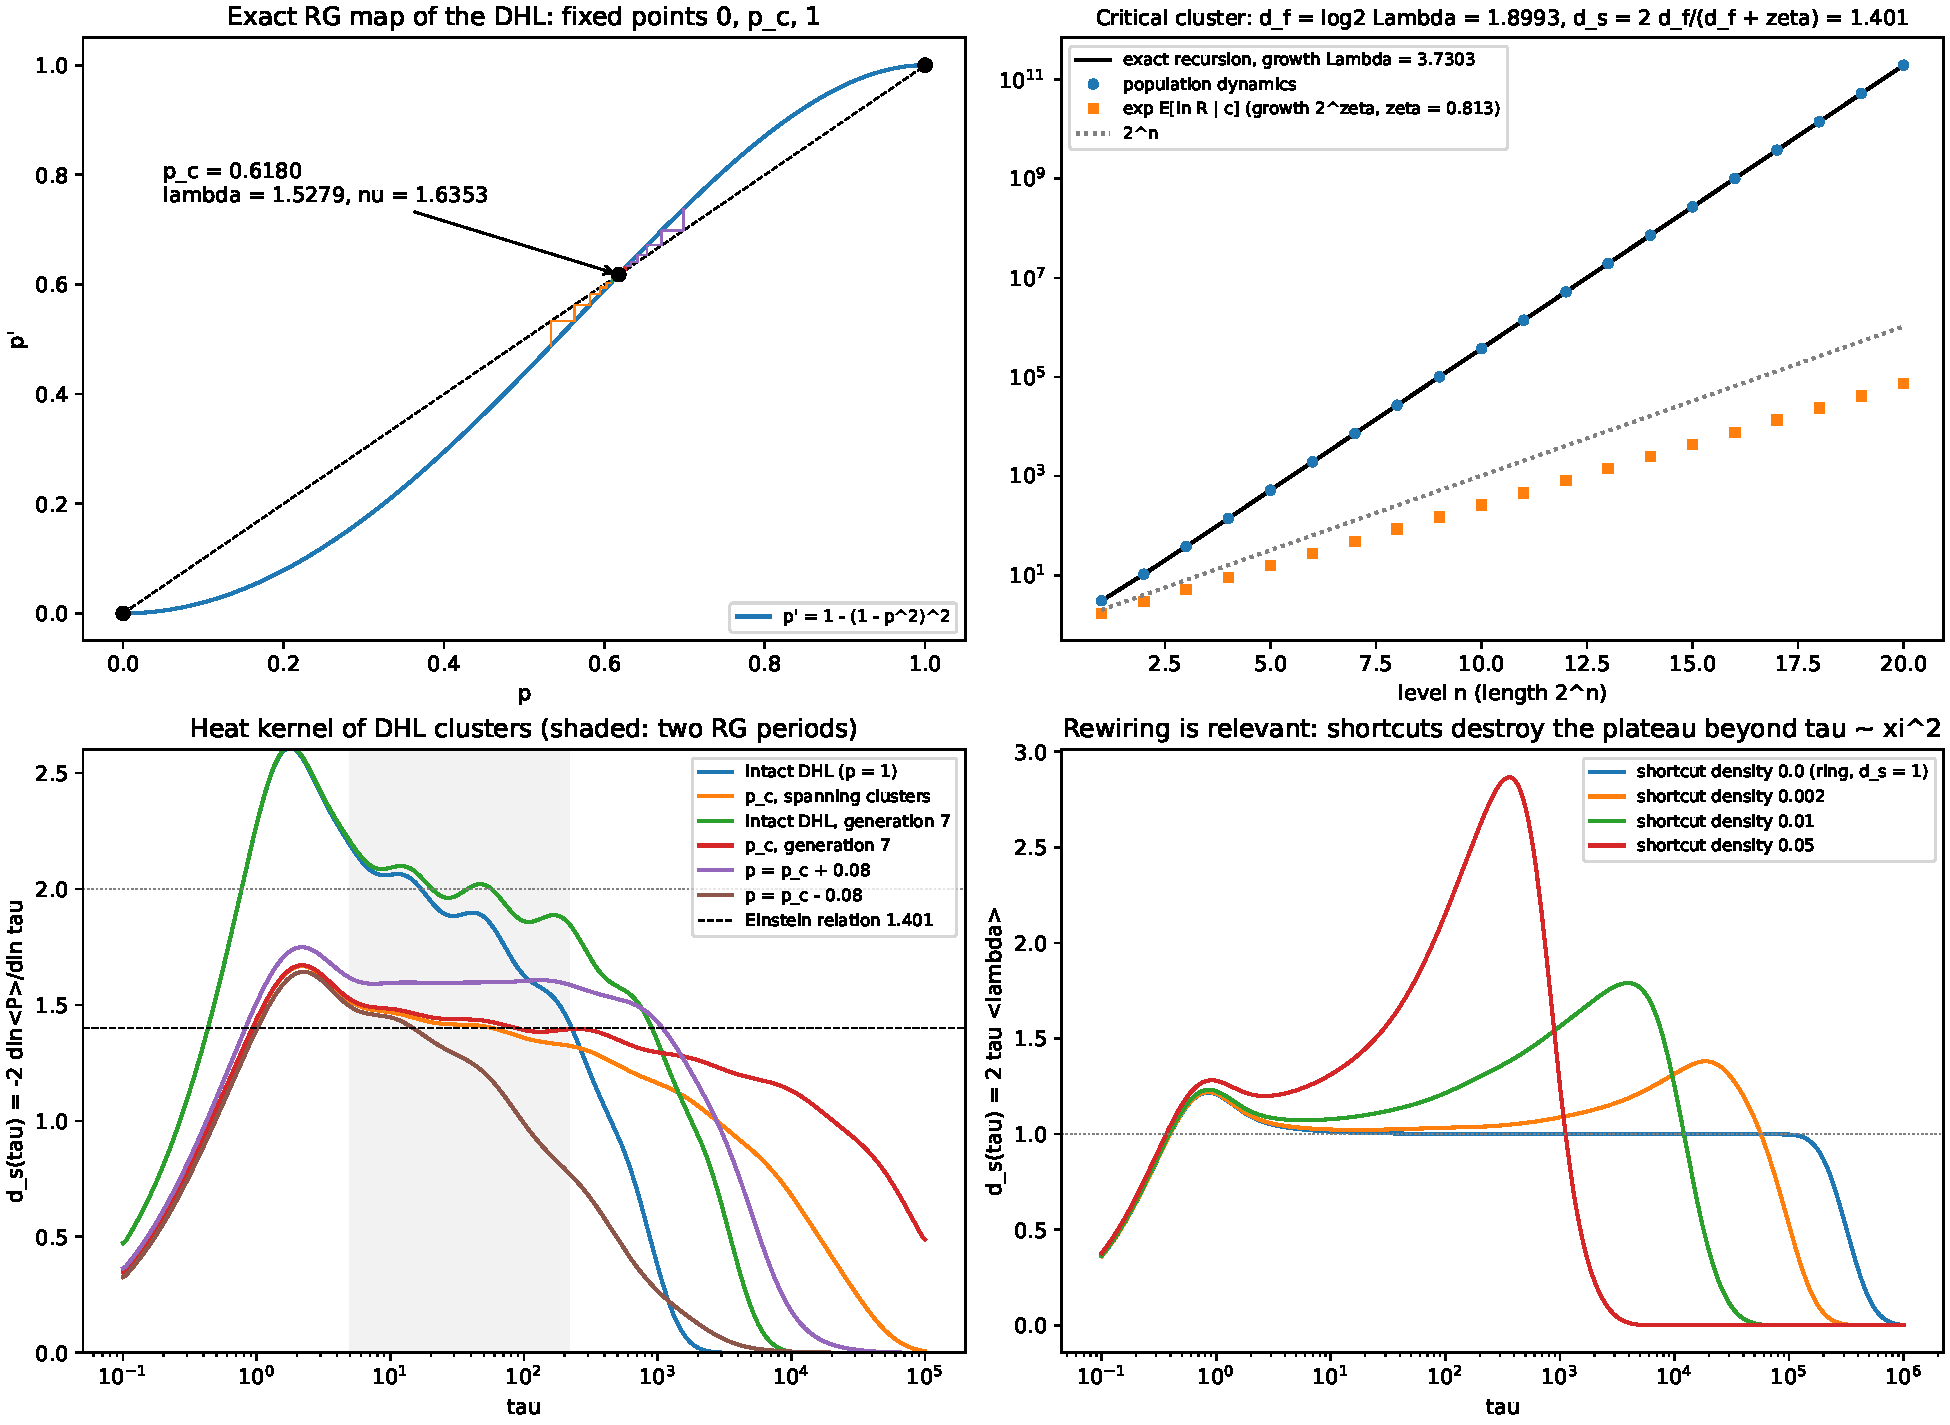
\includegraphics[width=\textwidth]{rg_spectral_dimension.pdf}
\caption{\emph{Top left:} exact RG map $p'=2p^2-p^4$ with cobweb flows away from $p_c$. \emph{Top right:} mean mass of
the critical spanning cluster from the exact recursion (line) and from population dynamics (dots), and
$\exp\EE[\ln R\mid c]$ for the resistance between the poles (squares), which grows as $2^{\zeta n}$ with $\zeta=0.813$, not as
$2^n$ (dotted). \emph{Bottom left:} $d_s(\tau)=-2\,\dd\ln\langle P\rangle/\dd\ln\tau$ from exact diagonalisation of the intact DHL and
of percolation clusters at and near $p_c$; the shaded window covers two RG periods; the dashed line is the Einstein
value $1.401$. \emph{Bottom right:} $d_s(\tau)=2\tau\langle\lambda\rangle_\tau$ for a ring of $2000$ sites with Newman--Watts
shortcuts.}
\label{fig:main}
\end{figure}

%=====================================================================
\section{Exact percolation renormalization on the diamond lattice}
\label{sec:rg}

The diamond hierarchical lattice $D_n$ is defined recursively~\cite{BerkerOstlund,HamblyKumagai}. $D_0$ is a single edge
between two poles. $D_{n+1}$ is obtained by replacing every edge of $D_n$ by a diamond: two branches in parallel, each
consisting of two edges in series. Equivalently, $D_{n+1}$ consists of four copies of $D_n$ arranged in a diamond. $D_n$
has $4^n$ edges and $\tfrac23(4^n+2)$ vertices, and the graph distance between the poles is $2^n$. The intact lattice has
mass dimension $2$. Its pole-to-pole resistance is independent of $n$, because two series edges in parallel with two
series edges have resistance one. Its spectral dimension is $2$, in the sense of eigenvalue counting~\cite{HamblyKumagai}.

Declare each edge open independently with probability $p$, and let $c_n$ be the event that the poles of $D_n$ are joined
by an open path. Since $D_{n+1}$ is made of four independent copies of $D_n$, $P(c_{n+1})=f(P(c_n))$ with
\begin{equation}
f(p)=1-(1-p^2)^2=2p^2-p^4 .
\label{eq:rgmap}
\end{equation}

\begin{proposition}
\label{prop:rg}
The map~\eqref{eq:rgmap} has fixed points $0$, $1$ and $p_c=(\sqrt5-1)/2$ in $[0,1]$. The first two are attracting and
$p_c$ is repulsive, with
\begin{equation}
\lambda=f'(p_c)=4p_c(1-p_c^2)=4p_c^2=6-2\sqrt5\approx1.5279,\qquad \nu=\frac{\ln2}{\ln\lambda}\approx1.6353 .
\end{equation}
\end{proposition}

\begin{proof}
$f(p)=p$ reduces to $p(p-1)(p^2+p-1)=0$. At $p_c$ we have $p_c^2=1-p_c$, hence $1-p_c^2=p_c$ and $f'(p_c)=4p_c^2=4(1-p_c)$.
$f'(0)=0$ and $f'(1)=0$. A deviation $\delta p$ grows by the factor $\lambda$ per level, i.e.\ per doubling of length, so
$\xi\sim|\delta p|^{-\nu}$ with $\nu=\ln2/\ln\lambda$.
\end{proof}

This is the standard percolation RG on the DHL~\cite{HamblyKumagai}. Its message for the question of
Section~\ref{sec:intro} is immediate. Every $p\neq p_c$ flows to $0$ or $1$, so a non-integer fixed point is reached
only by tuning one parameter.

%=====================================================================
\section{Closed-form mass dimension of the critical cluster}
\label{sec:mass}

Let $M_n$ be the number of open edges in the open cluster of pole $0$ in $D_n$. By symmetry, the cluster of pole $1$ has the
same law. Put
\begin{equation}
P_n=P(c_n),\qquad a_n=\EE[M_n\mathbf 1_{c_n}],\qquad b_n=\EE[M_n\mathbf 1_{\neg c_n}],
\end{equation}
with $(P_0,a_0,b_0)=(p,p,0)$ for a single edge.

\begin{lemma}[Series and parallel composition]
\label{lem:comp}
Let $X,Y$ be independent copies of a two-pole network with parameters $(P,a,b)$.
\begin{enumerate}
\item[(i)] Their series composition has $P_S=P^2$, $a_S=2Pa$ and $b_S=(1-P)a+(1+P)b$.
\item[(ii)] The parallel composition of two independent networks with parameters $(P_S,a_S,b_S)$ has
$P_Q=1-(1-P_S)^2$, $a_Q=2a_S+4P_Sb_S$ and $b_Q=2(1-P_S)b_S$.
\end{enumerate}
\end{lemma}

\begin{proof}
(i) Let $X$ join pole $0$ to the middle vertex $m$, and $Y$ join $m$ to pole $1$. The cluster of pole $0$ consists of the
cluster of pole $0$ in $X$, together with the cluster of $m$ in $Y$ if $X$ is crossed. So $M_S=M_X+\mathbf 1_{c_X}M'_Y$, where $M'_Y$
has the law of $M$ by symmetry. Hence $\EE[M_S\mathbf 1_{c_S}]=\EE[M_X\mathbf 1_{c_X}]P+P\,\EE[M'_Y\mathbf 1_{c_Y}]=2Pa$, and
$\EE M_S=(a+b)(1+P)$, which gives $b_S$.

(ii) If the parallel network is crossed, the poles lie in one cluster. A crossed branch contributes its pole cluster
$M_i$. An uncrossed branch contributes both of its pole clusters, $M_i+M'_i$, because the other branch joins the poles.
By independence of the branches,
$a_Q=\sum_i\bigl(\EE[M_i\mathbf 1_{c_i}]+\EE[(M_i+M_i')\mathbf 1_{\neg c_i}]\,P(c_j)\bigr)=2a_S+4P_Sb_S$, where $j\neq i$. If it is not crossed,
neither branch is, and $M_Q=M_1+M_2$, so $b_Q=2b_S(1-P_S)$.
\end{proof}

\begin{theorem}[Mass dimension]
\label{thm:mass}
At $p=p_c$ the vector $(a_n,b_n)$ obeys $(a_{n+1},b_{n+1})^{\mathsf T}=T\,(a_n,b_n)^{\mathsf T}$ with
\begin{equation}
T=\begin{pmatrix}12-4\sqrt5 & 2\sqrt5-2\\ 2\sqrt5-4 & 2\end{pmatrix}.
\label{eq:T}
\end{equation}
Its Perron eigenvalue is
\begin{equation}
\Lambda=7-2\sqrt5+\sqrt{73-32\sqrt5}=3.730288562\ldots,
\end{equation}
and the mean mass of the critical spanning cluster grows as $\EE[M_n\mid c_n]=a_n/p_c\sim C\,\Lambda^n$. Since the
pole distance is $2^n$, the mass dimension is
\begin{equation}
d_f=\log_2\Lambda=1.8992872\ldots
\end{equation}
\end{theorem}

\begin{proof}
Lemma~\ref{lem:comp} gives
$a_{n+1}=[4P+4P^2(1-P)]a_n+4P^2(1+P)b_n$ and $b_{n+1}=2(1-P^2)[(1-P)a_n+(1+P)b_n]$, with $P=P_n$. At $P=p_c$,
$p_c^2=1-p_c$ and $1-p_c^2=p_c$ give the entries~\eqref{eq:T}. The characteristic polynomial is
$x^2-(14-4\sqrt5)x+(4\sqrt5-4)$, whose larger root is $\Lambda$. $T$ has positive entries, and $(a_0,b_0)=(p_c,0)$ has a positive
component along the Perron vector. Hence $a_n\sim C\Lambda^n$ with $C>0$, and $P_n=p_c$ for all $n$.
\end{proof}

\begin{remark}[The skeleton]
Hambly and Kumagai describe the critical cluster through a multitype branching process. An edge is labelled $c$ if the
sub-diamond it represents is crossed~\cite{HamblyKumagai}. Given that its parent is crossed, an edge is crossed with
probability $p_c+(1-p_c)p_c^2$. The expected number of $c$-children of a $c$-edge is therefore $4(p_c+(1-p_c)p_c^2)=12-4\sqrt5$,
which is the entry $T_{11}$. The skeleton of edges that are $c$-labelled at every level thus has mass dimension
$\log_2(12-4\sqrt5)\approx1.6115$. It contains the current-carrying backbone and some, but not all, dangling edges.
\end{remark}

\paragraph{Check.} We simulate the recursion by population dynamics. At every level, the crossing indicator of each of
the four sub-networks is drawn exactly with probability $p_c$, and its mass and resistance are drawn from a pool of
$4\times10^5$ crossed or uncrossed samples of the previous level. Exact sampling of the indicator removes the drift that
the repulsive fixed point would otherwise cause. After $20$ levels the sampled mean mass is $1.9570\times10^{11}$,
against the exact $1.9583\times10^{11}$. The last growth ratio is $3.7287$, against $\Lambda=3.7303$
(Figure~\ref{fig:main}, top right).

%=====================================================================
\section{Resistance exponent and the critical spectral dimension}
\label{sec:ds}

\paragraph{Resistance.} Dangling parts carry no current, so the pole-to-pole resistance $R_n$ of a crossed cluster
satisfies the series and parallel laws. In series it is $R_X+R_Y$. In parallel it is $(R_1^{-1}+R_2^{-1})^{-1}$, with
$R=\infty$ for an uncrossed branch. The recursion is nonlinear, and $R_n/2^n$ does not converge. We define the resistance
exponent by the Lyapunov exponent
\begin{equation}
\zeta=\lim_{n\to\infty}\frac1n\,\EE\bigl[\log_2R_n\bigm|c_n\bigr] .
\end{equation}
In the population dynamics the increments of $\EE[\log_2R_n\mid c_n]$ are stationary from about level~$10$. Over the last
eight levels they give
\begin{equation}
\zeta=0.8127\pm0.0002 ,
\end{equation}
and the median of $R_n/2^n$ decreases geometrically ($0.128,0.112,0.099,0.087,0.076$ at levels $16$--$20$). The reason is
that, conditioned on a crossing, both branches are crossed with probability
$P_S^2/(1-(1-P_S)^2)=p_c^4/p_c=p_c^3=\sqrt5-2\approx0.236$. At such a level the resistance stays roughly the same
instead of doubling. Ignoring fluctuations this suggests $\zeta\approx1-0.236$; the fluctuations of the branch
resistances raise the value to $0.813$.

\paragraph{Einstein relation.} For a fractal with mass dimension $d_f$ and resistance exponent $\zeta$, the walk dimension is
$d_w=d_f+\zeta$ and the spectral dimension is $d_s=2d_f/d_w$~\cite{AlexanderOrbach,BenAvrahamHavlin}. Hence
\begin{equation}
d_s=\frac{2d_f}{d_f+\zeta}=\frac{2\times1.89929}{1.89929+0.8127}\approx1.401 .
\label{eq:einstein}
\end{equation}
This combines an annealed mass exponent with a typical resistance exponent. We therefore test it directly.

\paragraph{Exact diagonalisation.} We sample bond configurations of $D_6$ ($4096$ edges) and $D_7$ ($16384$ edges) at $p_c$
and keep the cluster of pole $0$ when it reaches pole $1$. For each sample we compute the full spectrum of the
combinatorial graph Laplacian. From the annealed return probability
$\langle P(\tau)\rangle=\langle V^{-1}\mathrm{Tr}\,e^{-\tau\Delta}\rangle$ we obtain $d_s(\tau)=-2\,\dd\ln\langle P\rangle/\dd\ln\tau$. For a single
graph this is $2\tau\langle\lambda\rangle_\tau$~\cite{Chen2026_qgc}. The curves oscillate log-periodically. One RG level multiplies
time by $\Lambda2^\zeta=6.552$, so we average $d_s$ uniformly in $\ln\tau$ over exactly two periods, $5\le\tau\le215$. The intact
lattice, whose exact value is $2$, calibrates the finite-size error. We also compute the quenched average, the mean over
samples of $2\tau\langle\lambda\rangle_\tau$. Table~\ref{tab:ds} shows the results.

\begin{table}[ht]
\centering
\caption{Spectral dimension averaged uniformly in $\ln\tau$ over two RG periods ($5\le\tau\le215$), from the annealed
return probability and as a quenched average over samples.}
\label{tab:ds}
\begin{tabular}{lrrrr}
\toprule
Graph & samples & mean size & annealed & quenched \\
\midrule
intact DHL, $D_6$ & 1 & 2732 & 1.860 & 1.860 \\
intact DHL, $D_7$ & 1 & 10924 & 1.994 & 1.994 \\
critical spanning cluster, $D_6$ & 60 & 1791 & 1.412 & 1.414 \\
critical spanning cluster, $D_7$ & 24 & 6567 & 1.438 & 1.439 \\
\midrule
Einstein relation~\eqref{eq:einstein} & & & \multicolumn{2}{c}{1.401} \\
\bottomrule
\end{tabular}
\end{table}

On $D_7$ the intact lattice is within $0.006$ of its exact value, so the generation-$7$ estimate is reliable to a few
hundredths. We conclude that the full critical spanning cluster has
\begin{equation}
d_s\approx1.40\text{--}1.44 .
\end{equation}
The annealed and quenched averages agree to $0.002$, so the choice of ensemble average is immaterial here. The
residual difference from~\eqref{eq:einstein}, which combines an annealed mass exponent with a typical resistance
exponent, is of the size of the finite-size error on $D_6$ and the sampling error on $D_7$. The value $1.25$ is excluded.

%=====================================================================
\section{RG stability and crossovers}
\label{sec:stability}

\paragraph{Off-critical flows.} For $p=p_c\pm\delta$ the deviation grows by the factor $\lambda$ per level. At scales below
$\xi\sim\delta^{-\nu}$ the cluster looks critical, and above $\xi$ it flows to the intact lattice ($d_s\to2$) or to finite
fragments ($d_s\to0$). For $\delta=0.08$, $\xi\approx0.08^{-1.635}\approx62$, which is comparable to the size $2^6=64$ of $D_6$.
Accordingly, at $p_c-0.08$ the curve $d_s(\tau)$ falls towards $0$ inside the window. At $p_c+0.08$ it stays near $1.60$,
between the critical and the intact values. At fixed $\tau$, $d_s$ changes continuously with $p$. Only the asymptotic
exponent, $0$, $d_s^{(c)}$ or $2$, is discontinuous at $p_c$. The ``jump'' is a crossover.

\paragraph{Rewiring.} The other perturbation proposed for geometric RG flows is rewiring. Add to a ring of $N=2000$ sites a
Poisson number, with mean $\phi N$, of random shortcuts (Newman--Watts model~\cite{WattsStrogatz,NewmanWatts}). The typical
distance between shortcut ends is $\xi=1/\phi$, which is relevant with $\nu=1$~\cite{NewmanWatts}. The ring has
$d_s=1$, with a small lattice overshoot to $1.218$, the value $1.2178\,d$ found in~\cite{Chen2026_qgc}. With shortcuts,
$d_s(\tau)=2\tau\langle\lambda\rangle_\tau$ rises above $1$ for $\tau\gtrsim\xi^2$. Its maximum is $1.38$, $1.79$ and $2.87$ for $\phi=0.002,0.01,0.05$
before finite-size collapse (Figure~\ref{fig:main}, bottom right). Rewiring therefore drives the graph away from any
finite-dimensional plateau. It does not stabilise a non-integer value.

%=====================================================================
\section{Transport universality}
\label{sec:universality}

Table~\ref{tab:compare} collects the exponents of critical percolation clusters on several lattices.

\begin{table}[ht]
\centering
\caption{Mass dimension, resistance exponent and spectral dimension. Exponents are with respect to the Euclidean or
hierarchical length; for the Hambly--Kumagai diffusion, $\theta$ is the dimension in its effective-resistance metric.}
\label{tab:compare}
\begin{tabular}{lcccl}
\toprule
Object & $d_f$ & $\zeta$ & $d_s$ & Source \\
\midrule
intact DHL & $2$ & $0$ & $2$ & exact \\
DHL critical spanning cluster & $1.89929$ & $0.8127(2)$ & $1.40$--$1.44$ & this work \\
DHL skeleton, renormalised form & \multicolumn{2}{c}{$\theta=5.2654$} & $2\theta/(\theta+1)\approx1.681$ & \cite{HamblyKumagai} \\
$\ZZ^2$ critical percolation & $91/48$ & $0.9826(8)$ & $1.317$ & \cite{Grassberger,StaufferAharony} \\
mean field ($d>6$) & $4$ & $2$ & $4/3$ & \cite{AlexanderOrbach,KozmaNachmias} \\
\bottomrule
\end{tabular}
\end{table}

Three conclusions follow.
\begin{enumerate}
\item \emph{Geometry is not transport.} The DHL cluster reproduces the mass dimension of two-dimensional percolation
to $0.2\%$ ($1.8993$ against $1.8958$). Its resistance exponent, however, is $0.813$ against $0.983$, and its spectral
dimension is about $1.40$ against $1.317$. Migdal--Kadanoff-type hierarchical lattices approximate the geometric
exponents of $\ZZ^2$, but they are not in its transport universality class. Within the DHL the lower resistance
exponent has a simple source (Section~\ref{sec:ds}). Conditioned on a crossing, both branches of a diamond are crossed
with probability $p_c^3=\sqrt5-2$ at every level, independently of scale, and such levels do not increase the
resistance. On $\ZZ^2$, loops of all shapes and sizes contribute, and we do not claim a comparable mechanism there.
\item \emph{``The'' critical cluster is not unique.} Hambly and Kumagai construct a diffusion on the scaling limit of the
$c$-labelled skeleton. Its Dirichlet form is renormalised so that the resistance across the lattice stays one, and its
natural measure is the one carried by the branching process. In the resulting resistance metric they prove heat-kernel
bounds with exponent $\theta/(\theta+1)$, $\theta=5.2654$, i.e.\ spectral dimension $\approx1.681$~\cite{HamblyKumagai}. This
is a different subgraph, measure and Laplacian from the full cluster with unit conductances. The difference of
$1.68$ and $1.40$ shows that the spectral dimension depends on these choices, not only on the lattice.
\item \emph{Mean field is not two-dimensional.} The Alexander--Orbach value $4/3$ is proved in high
dimensions~\cite{KozmaNachmias}. Neither the $\ZZ^2$ value nor the DHL value equals it, and none equals $1.25$.
\end{enumerate}

%=====================================================================
\section{Discussion and conclusion}
\label{sec:conclusion}

In a model where the coarse-graining of a graph is exact, the spectral dimension behaves as RG theory predicts. Integer
values ($2$, and $0$ for fragments) are attracting fixed points. A non-integer value, $d_s\approx1.40$ for the full DHL
critical cluster, occurs only at the repulsive fixed point $p_c$ and must be tuned. The change from integer to
non-integer behaviour is a crossover at $\xi\sim|p-p_c|^{-\nu}$, not a jump. The critical value is determined by two
exponents. The mass exponent has the closed form $\log_2\bigl(7-2\sqrt5+\sqrt{73-32\sqrt5}\bigr)$, and the resistance exponent
$0.8127$ is a Lyapunov exponent of a nonlinear recursion. Rewiring is a relevant perturbation that removes rather than
creates non-integer plateaus.

This has two consequences for applications. In quantum gravity, a non-integer spectral dimension produced by a
critical point of a geometric RG requires the tuning of a relevant coupling, as for the second-order transition lines
of causal dynamical triangulations~\cite{AJL}. Its value depends on the transport properties of the critical geometry
and on the Laplacian used, not only on its mass dimension. In biological growth, claims of a common ``universality
class'' for fractal tissues or leaf margins would require an RG in which the relevant directions are identified and
the transport exponents are measured. A fractal box-counting dimension alone does not determine the spectral
dimension, as Table~\ref{tab:compare} shows. A stable non-integer $d_s$ would need a mechanism that makes the critical
point attractive, such as self-organised criticality. This is a hypothesis to be tested, not a consequence of
coarse-graining.

\section*{Data and code availability}
The script \texttt{rg\_spectral\_dimension.py}, the data (CSV), the figure and the console output are available at
\url{https://github.com/Ruqing1963/rg-spectral-dimension} and archived under DOI \href{https://doi.org/\paperdoi}{\paperdoi}.

%=====================================================================
\begingroup\raggedright
\begin{thebibliography}{99}\small
\bibitem{AJL} J.~Ambj{\o}rn, J.~Jurkiewicz, R.~Loll, ``Spectral dimension of the universe is scale dependent'', Phys.\ Rev.\ Lett.\ 95 (2005) 171301, arXiv:hep-th/0505113.
\bibitem{Carlip} S.~Carlip, ``Dimension and dimensional reduction in quantum gravity'', Class.\ Quantum Grav.\ 34 (2017) 193001, arXiv:1705.05417.
\bibitem{BenAvrahamHavlin} D.~ben-Avraham, S.~Havlin, \emph{Diffusion and Reactions in Fractals and Disordered Systems}, Cambridge University Press (2000).
\bibitem{Chen2026_qgc} R.~Chen, ``Crossover from discrete to continuous quantum geometry: Running spectral dimensions, noncommutative spectral triples, and critical phase transitions'' (2026), doi:10.5281/zenodo.23195881.
\bibitem{BerkerOstlund} A.~N.~Berker, S.~Ostlund, ``Renormalisation-group calculations of finite systems: order parameter and specific heat for epitaxial ordering'', J.\ Phys.\ C 12 (1979) 4961.
\bibitem{KaufmanGriffiths} M.~Kaufman, R.~B.~Griffiths, ``Exactly soluble Ising models on hierarchical lattices'', Phys.\ Rev.\ B 24 (1981) 496.
\bibitem{HamblyKumagai} B.~M.~Hambly, T.~Kumagai, ``Diffusion on the scaling limit of the critical percolation cluster in the diamond hierarchical lattice'', Commun.\ Math.\ Phys.\ 295 (2010) 29--69, doi:10.1007/s00220-009-0981-3.
\bibitem{AlexanderOrbach} S.~Alexander, R.~Orbach, ``Density of states on fractals: `fractons'\,'', J.\ Physique Lett.\ 43 (1982) L625--L631.
\bibitem{WattsStrogatz} D.~J.~Watts, S.~H.~Strogatz, ``Collective dynamics of `small-world' networks'', Nature 393 (1998) 440--442.
\bibitem{NewmanWatts} M.~E.~J.~Newman, D.~J.~Watts, ``Renormalization group analysis of the small-world network model'', Phys.\ Lett.\ A 263 (1999) 341--346, arXiv:cond-mat/9903357.
\bibitem{Grassberger} P.~Grassberger, ``Conductivity exponent and backbone dimension in 2-d percolation'', Physica A 262 (1999) 251, arXiv:cond-mat/9808095.
\bibitem{StaufferAharony} D.~Stauffer, A.~Aharony, \emph{Introduction to Percolation Theory}, 2nd ed., Taylor \& Francis, London (1994).
\bibitem{JonssonWheater} T.~Jonsson, J.~F.~Wheater, ``The spectral dimension of the branched polymer phase of two-dimensional quantum gravity'', Nucl.\ Phys.\ B 515 (1998) 549--574, arXiv:hep-lat/9710024.
\bibitem{KozmaNachmias} G.~Kozma, A.~Nachmias, ``The Alexander--Orbach conjecture holds in high dimensions'', Invent.\ Math.\ 178 (2009) 635--654, arXiv:0806.1442.
\end{thebibliography}
\endgroup

\end{document}
